\begin{figure}[htbp]
\section*{ABCB7}
\centering
\begin{subfigure}[b]{0.95\textwidth}
\centering
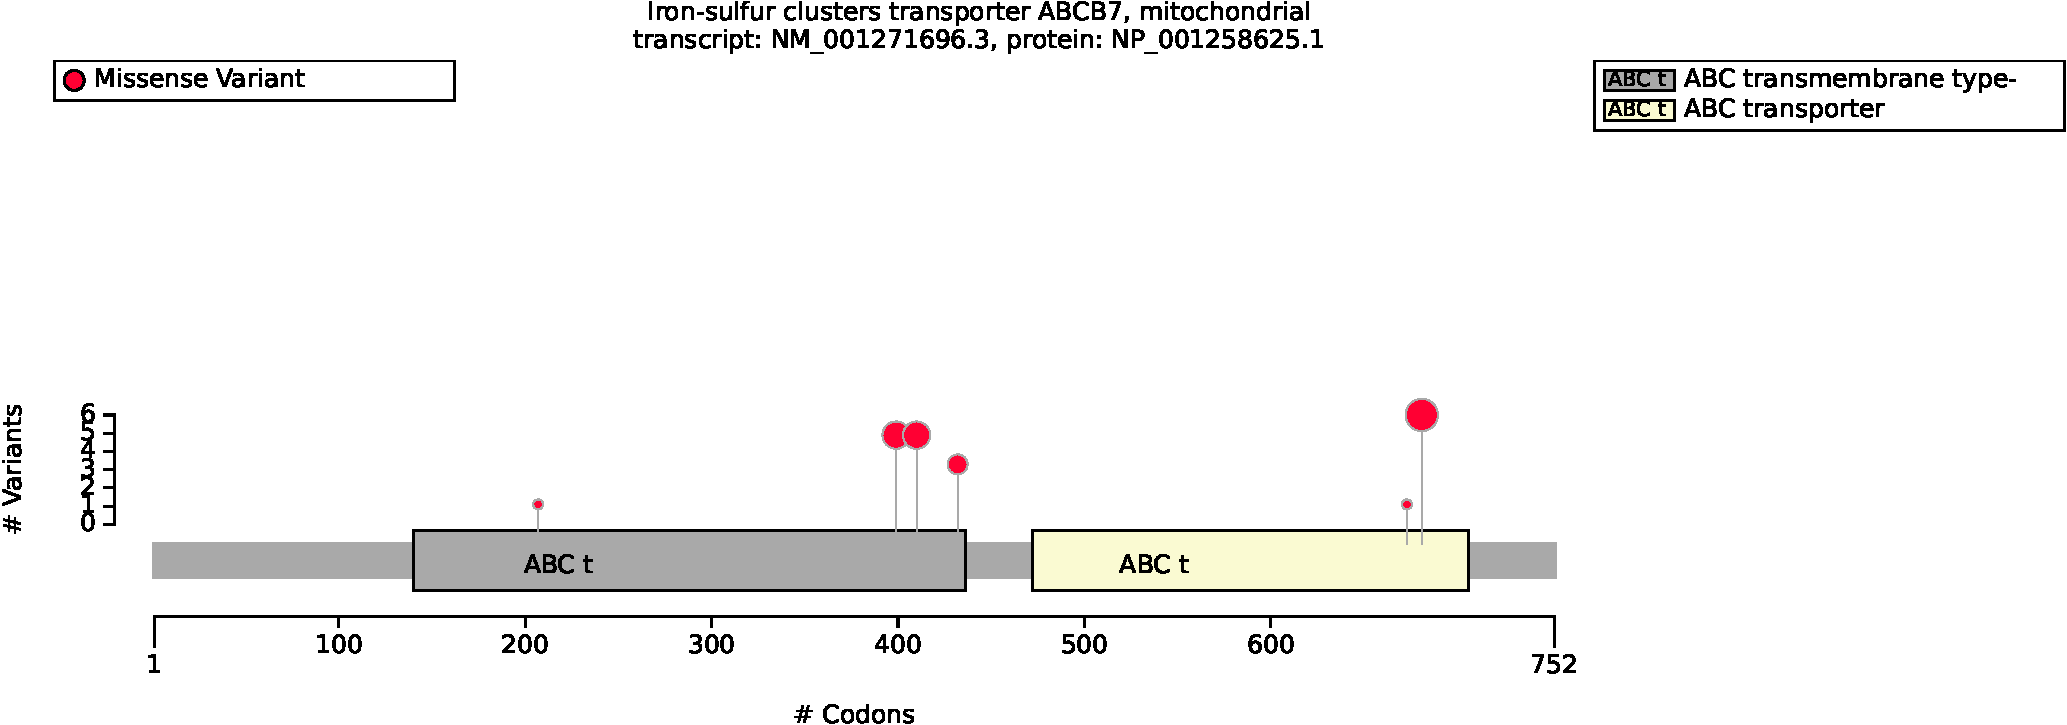
\includegraphics[width=\textwidth]{ img/ABCB7_protein_diagram.pdf} 
\captionsetup{justification=raggedright,singlelinecheck=false}
\caption{Distribution of variants in ABCB7}
\end{subfigure}

\vspace{2em}

\begin{subfigure}[b]{0.95\textwidth}
\centering
\resizebox{\textwidth}{!}{
\begin{tabular}{llllrr}
\toprule
Genotype (A) & Genotype (B) & total tests performed & significant results\\
\midrule
ABC transmembrane type-1 & Other region & 12 & 0\\
p.Gly682Ser & Other variant & 10 & 0\\
\bottomrule
\end{tabular}
}
\captionsetup{justification=raggedright,singlelinecheck=false}
\caption{Fisher Exact Test performed to compare HPO annotation frequency with respect to variants located in the
ABC transmembrane type-1 region and p.Gly682Ser.}
\end{subfigure}

\vspace{2em}

\caption{ The cohort comprised 18 individuals (0 females, 18 males). A total of 52 HPO terms were used to annotate the cohort. Disease diagnosis: Anemia, sideroblastic, and spinocerebellar ataxia (OMIM:301310). No statistically significant results identified. A total of 18 unique variant alleles were found in \textit{ABCB7} (transcript: \texttt{NM\_001271696.3}, protein id: \texttt{NP\_001258625.1}).}
\end{figure}
